% Chapter Template

\chapter{Using STUFF to do THINGS} % Main chapter title

\label{Chapter5} % Change X to a consecutive number; for referencing this chapter elsewhere, use \ref{ChapterX}

%-----------------------------------------------------------
\section{Introduction}
%-----------------------------------------------------------

Many variables affect heat flux across core-mantle boundary (CMB). On the mantle side, they are the properties of the thermal boundary layer (TBL); the chemistry, temperature, and thickness. As explained in Chapter~\ref{Chapter4}, \tcs is dependent on the temperature and composition of a mineral. The thermal gradient away from the CMB depends on the thickness and temperature at the top and bottom of the TBL. Recalling Fourier's law once more, heat flux ($q$) is equal to the product of the thermal conductivity ($\kappa$), and the temperature gradient ($\nabla{T}$)
%
\begin{equation}
q=-\kappa \nabla{T}\ . 
\label{eq:fourier5}
\end{equation}

%---------------------------------------
\subsection{Approaching the problem}
%---------------------------------------

A simple one-dimensional model is not sufficient to describe the Earth, recalling Section~\ref{sec:LM}, two large low shear velocity provinces (LLSVPs) sit approximately on opposite sides of the CMB. A two-dimensional model, around the equator perhaps, would better describe the situation, but the CMB is spherical. A more sophisticated model is required to model changes in CMB structure with varying latitude and longitudes.

%---------------------------------------
\subsection{Introducing LEMA}
%---------------------------------------

!!! Need to introduce LEMA



%-----------------------------------------------------------
\section{Methodology}
%-----------------------------------------------------------

Using LEMA, I specify a CMB base condition, and a TBL condition at some height above it. In all models I consider the CMB will be isothermal, due to the considerably faster nature of core dynamics compared to those on the mantle side \citep[e.g.][]{Gibbons2000}. The TBL will have a variable mean temperature, and regions of higher and lower temperature. The lower mantle has an average Fe\%, but the LLSVPs are enriched compared the depleted surrounding bulk lower mantle. By varying the temperature and composition at the CMB, conductivity can be altered using the model from Section~\ref{sec:kappa_model}. The difference in temperature between CMB and TBL, and the undulations on the latter, control the lower mantle temperature gradient. 

The magnitude of the heat flux will change with position on the CMB, as the TBL characteristics change. Lateral variations can show how heat flux is sensitive to the lower mantle conditions, and what condition or combination of conditions is most significant. The calculated heat flux and lateral variations can then be compared to observables, dismissing scenarios which are unfeasible or unstable. There are many variables to consider in the lower mantle, and observables to compare to. The variable conductivities from Chapter~\ref{Chapter4} will play an important role in constraining CMB heat flux.

%---------------------------------------
\subsection{Using spherical harmonics to replicate CMB features}
%---------------------------------------

I can use spherical harmonics to generate structures that resemble LLSVPs. The centre of LLSVPs are approximately located on the equator, antipodal at $0\degsym$ and $180\degsym$ longitude (the African and Pacific LLSVPs respectively). A first order approxiamtion for this geometry is the spherical harmonic $Y^{2}_{2}$, four quadrants of varying polarity around the polar axis. This looks good, but the projection is misleading in that it actually extends to the poles. It can be improved by stacking $Y^{0}_{2}$ on top of it, enhancing regions on the equator and reducing everything towards the poles. The results is two circular patterns, each located at opposite sides of the equator.

%$Y^{m}_{l}$

\begin{figure}[h]
  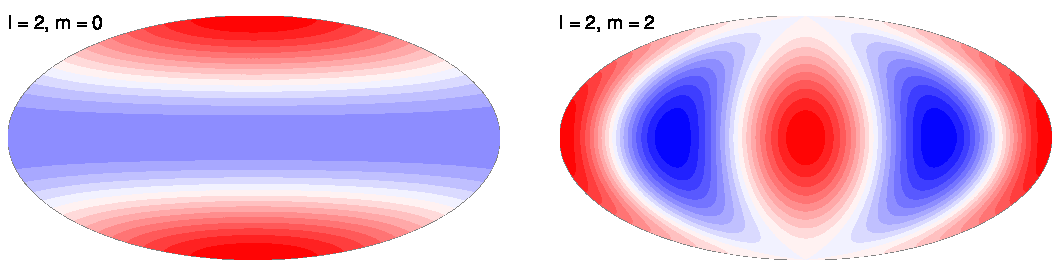
\includegraphics[width=\linewidth]{Figures/sph_harm.png}
  \caption[SPHERICAL HARMONICS]{Source: http://www-udc.ig.utexas.edu/external/becker/teaching-sh.html
  
These two harmonics are added together, amplifying blue regions on the equator, and diminshing everything else.}
  \label{fig:spherical_harmonics_diagram}
\end{figure}

For the $Y^{2}_{2}$ pattern, the areas of positive and negative amplitude regions are equal. For the  $Y^{0}_{2}$-combined model, the distribution of polarities is not even. By the way something like temperature is set up in the model, having a mean value with a ``$\pm$'' range leads to hotter hots, and warmer colds. There is more of the cold, surrounding mantle compared to LLSVP-designated regions, so the LLSVPs have to be hotter than the surrounding mantle is colder.



%---------------------------------------
\subsection{Modelling heat flux in the lower mantle}
%---------------------------------------

Conductivity cannot be probed from the surface, but seismic velocities can be inferred from tomography. The same processes that affect conductivity generally affect shear wave velocity in the same fashion, be it increase or decrease. I can use $V_{\mathrm{S}}$ observations as an analogue to make inferences about the lower mantle \tc.

When conductivity is kept constant across the whole CMB, variations in heat flux are determined solely by the lower mantle temperature profile. The reverse is also true, with constant temperature gradient above the CMB, conductivity controls lateral heat flow variations. This is a vast oversimplification, just talking about possible endmembers, in reality there will be both temperature and compositional factors affecting heat flux. Conductivity itself is temperature-dependent, further tying the two variables together.

When modelling LLSVPs, we are assuming they are thermochemical piles, that they are hotter and denser (e.g. high Fe\%) than the surrounding lower mantle. Increasing temperature reduces conductivity, as does increasing impurity inclusion (up to the turning point, recall Section~\ref{sec:kc_turning _point}). By modelling LLSVPs as purely thermal piles (i.e. increasing their temperature), we see a reduction in heat flux. This flux is further reduced when Fe content is increased, as conductivity decreases with impurity content. By altering temperature and composition in tandem, I will be able to generate sets of lower mantle conditions to compare with observations.



%---------------------------------------
\subsection{Lateral variations in heat flux}
%---------------------------------------

While this model is of dubious use in constraining the exact nature of CMB heat flux, inferences can be made on the relative lateral variations. How much heat is impeded passing through a LLSVP? How extreme do temperature and compositional variations need to be to significantly affect the distribution of heat flow? I can determine the lateral variation in heat flux as
%
\begin{equation}
\label{eq.q_star}
q* = \frac{q_{\mathrm{max}}-q_{\mathrm{min}}}{q_{\mathrm{mean}}}\ ,
\end{equation}
%
where max and min refer to the calculated extremes, and mean the average over the whole CMB. The larger the value of $q*$, the smaller the heat flux through the LLSVPs (which are hotter and denser, having the effect of reducing \tc). While the magnitudes of heat flux may not be accurate, using $q*$ will let me make comments on the significance of thermal conductivity in the Earth's heat engine for a wide range of possible lower mantle conditions.

%-----------------------------------------------------------
\section{Notes}
%-----------------------------------------------------------

VARIABLES TO PLAY WITH

Temp-cmb,
Temp-tbl,
Temp-diff,
Temp-hot,
Temp-cold,

Height-tbl,
Height-llsvp (peak height, how is shape considered, sph. harm.?)

Comp-mean,
Comp-lm,
Comp-llsvp,


The things I can vary are temperature, composition, and TBL thickness. Temperature and thickness amount to the same thing in the model however, which is the thermal gradient.

Temperature variations are set at the top of the model (1000~km above CMB). The temperature is constant all the way down to the TBL, at which it increases up to the CMB temperature. I only need to plot the temperature gradient at the CMB. WHAT IS THE POINT OF THE TBL THEN? OR RATHER, WHAT IS THE POINT OF MANTLE ABOVE THE TBL?

In the real world, Fe may be localised. in the model, it is constant radially up. 

I need to fiddle with parameters to obtain realistic change in shear velocity. I can then record this and q* ``about 2\% shear wave anomaly'' - vary temp to get this, then comp, then both

Changing temperature at the top of the model changes gradient. Changing temperature at the bottom also changes conductivity.

Keep the top around 1000~K cooler?

Turn notebook into function with input arguments, then run in a loop.

Investigate thermo mantle, chemical mantle, and then thermochemical. How sensible are these models? How feasible are they?

Lateral temperature variations are different to radial variations!

use model to link tomography

what range could q* occupy, and why would jon and chris care?




PLAN


LEMA - what is, why am i using it, how does it work ``i will use LEMA to explore'' - numerical tests

CHEBYSHEVYS related to LEMA section? -numerical tests ``1D CMB heat flux''

Future work / conclusion / caveats / limitations. i am only using \bdg, future work would be to add MgO















